\documentclass[tikz,border=6pt]{standalone}
\usepackage{amsmath,amssymb}
\usepackage{xcolor}
\definecolor{accent}{HTML}{A13D2C}
\definecolor{accent2}{HTML}{2B5F6B}
\definecolor{muted}{HTML}{5A564F}
\definecolor{linecol}{HTML}{D8D2C4}
\definecolor{astroblue}{HTML}{1B4F72}
\definecolor{sunyellow}{HTML}{E8A33D}
\usetikzlibrary{calc,arrows.meta,decorations.pathreplacing}
\usepackage[T1]{fontenc}\usepackage{newpxtext,newpxmath}  % same fonts as the notes
\begin{document}
% Thin-lens geometry for a source directly behind a point lens. Angles exaggerated.
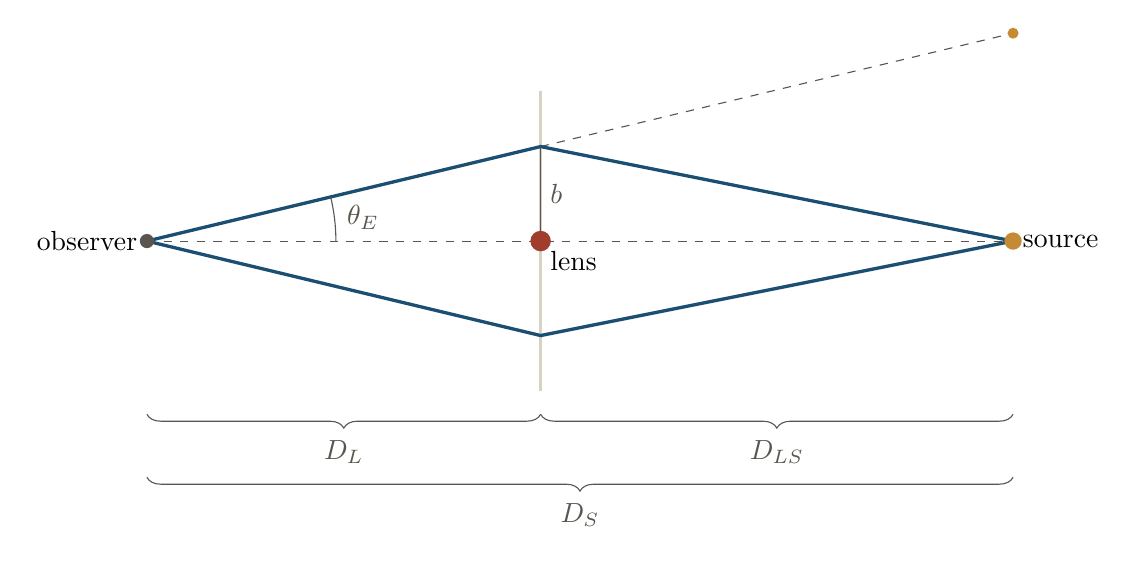
\begin{tikzpicture}[x=1cm,y=1cm, >={Stealth[length=2.4mm]}]
  \coordinate (O) at (0,0);
  \coordinate (L) at (5,0);
  \coordinate (S) at (11,0);
  \coordinate (B) at (5,1.2);
  \coordinate (Bm) at (5,-1.2);
  \draw[muted, dashed] (O) -- (S);
  \draw[linecol, line width=0.9pt] (5,-1.9) -- (5,1.9);
  % apparent direction, continued past the lens plane
  \draw[muted, dashed] (B) -- ($(O)!11/5!(B)$);
  % rays from the source to the observer, bent at the lens plane
  \draw[astroblue, line width=1.2pt] (S) -- (B) -- (O);
  \draw[astroblue, line width=1.2pt] (S) -- (Bm) -- (O);
  \draw[muted] (L) -- (B) node[midway, right] {$b$};
  % angle at observer
  \draw[muted] (2.4,0) arc (0:{atan(1.2/5)}:2.4); \node[muted, right] at (2.42,0.3) {$\theta_E$};
  \fill[muted] (O) circle (0.09);
  \fill[accent] (L) circle (0.13);
  \fill[sunyellow!85!black] (S) circle (0.11);
  \fill[sunyellow!85!black] ($(O)!11/5!(B)$) circle (0.07);
  \node[left] at (O) {observer};
  \node[below right] at (L) {lens};
  \node[right] at (S) {source};
  % distances
  \draw[decorate, decoration={brace, mirror, amplitude=5pt}, muted] (0,-2.2) -- (5,-2.2) node[midway, below=6pt] {$D_L$};
  \draw[decorate, decoration={brace, mirror, amplitude=5pt}, muted] (5,-2.2) -- (11,-2.2) node[midway, below=6pt] {$D_{LS}$};
  \draw[decorate, decoration={brace, mirror, amplitude=5pt}, muted] (0,-3.0) -- (11,-3.0) node[midway, below=6pt] {$D_S$};
\end{tikzpicture}
\end{document}
